\documentclass[12pt]{article}
\usepackage{setspace}   % paquete para interlineado
\usepackage{newtxtext,newtxmath} % Times New Roman

%otra opcion para times roman adaptable a versiones
%\usepackage{mathptmx}

%haber si funciona mas parecido a word
\setstretch{1.5}  
%\usepackage[protrusion,expansion]{microtype}
%\onehalfspacing               % interlineado 1.5
\usepackage{amsmath} % Para usar \text{}
\usepackage[utf8]{inputenc}
\usepackage[spanish]{babel}
\usepackage[letterpaper, left=3cm, right=2.5cm, top=2.5cm, bottom=2.5cm]{geometry}
\usepackage{graphicx}
\usepackage{titlesec}
\usepackage{setspace}
\usepackage{lipsum}
\geometry{margin=1in}


%%%%%%%% PARA VINCULOSs%%%%%
\usepackage[hidelinks]{hyperref}
\usepackage{pdfpages}



%PAQUETE para incluir PDF´s
\usepackage{pdfpages} % para incluir PDFs


\begin{document}
	%-----------------CARATULA-------------
	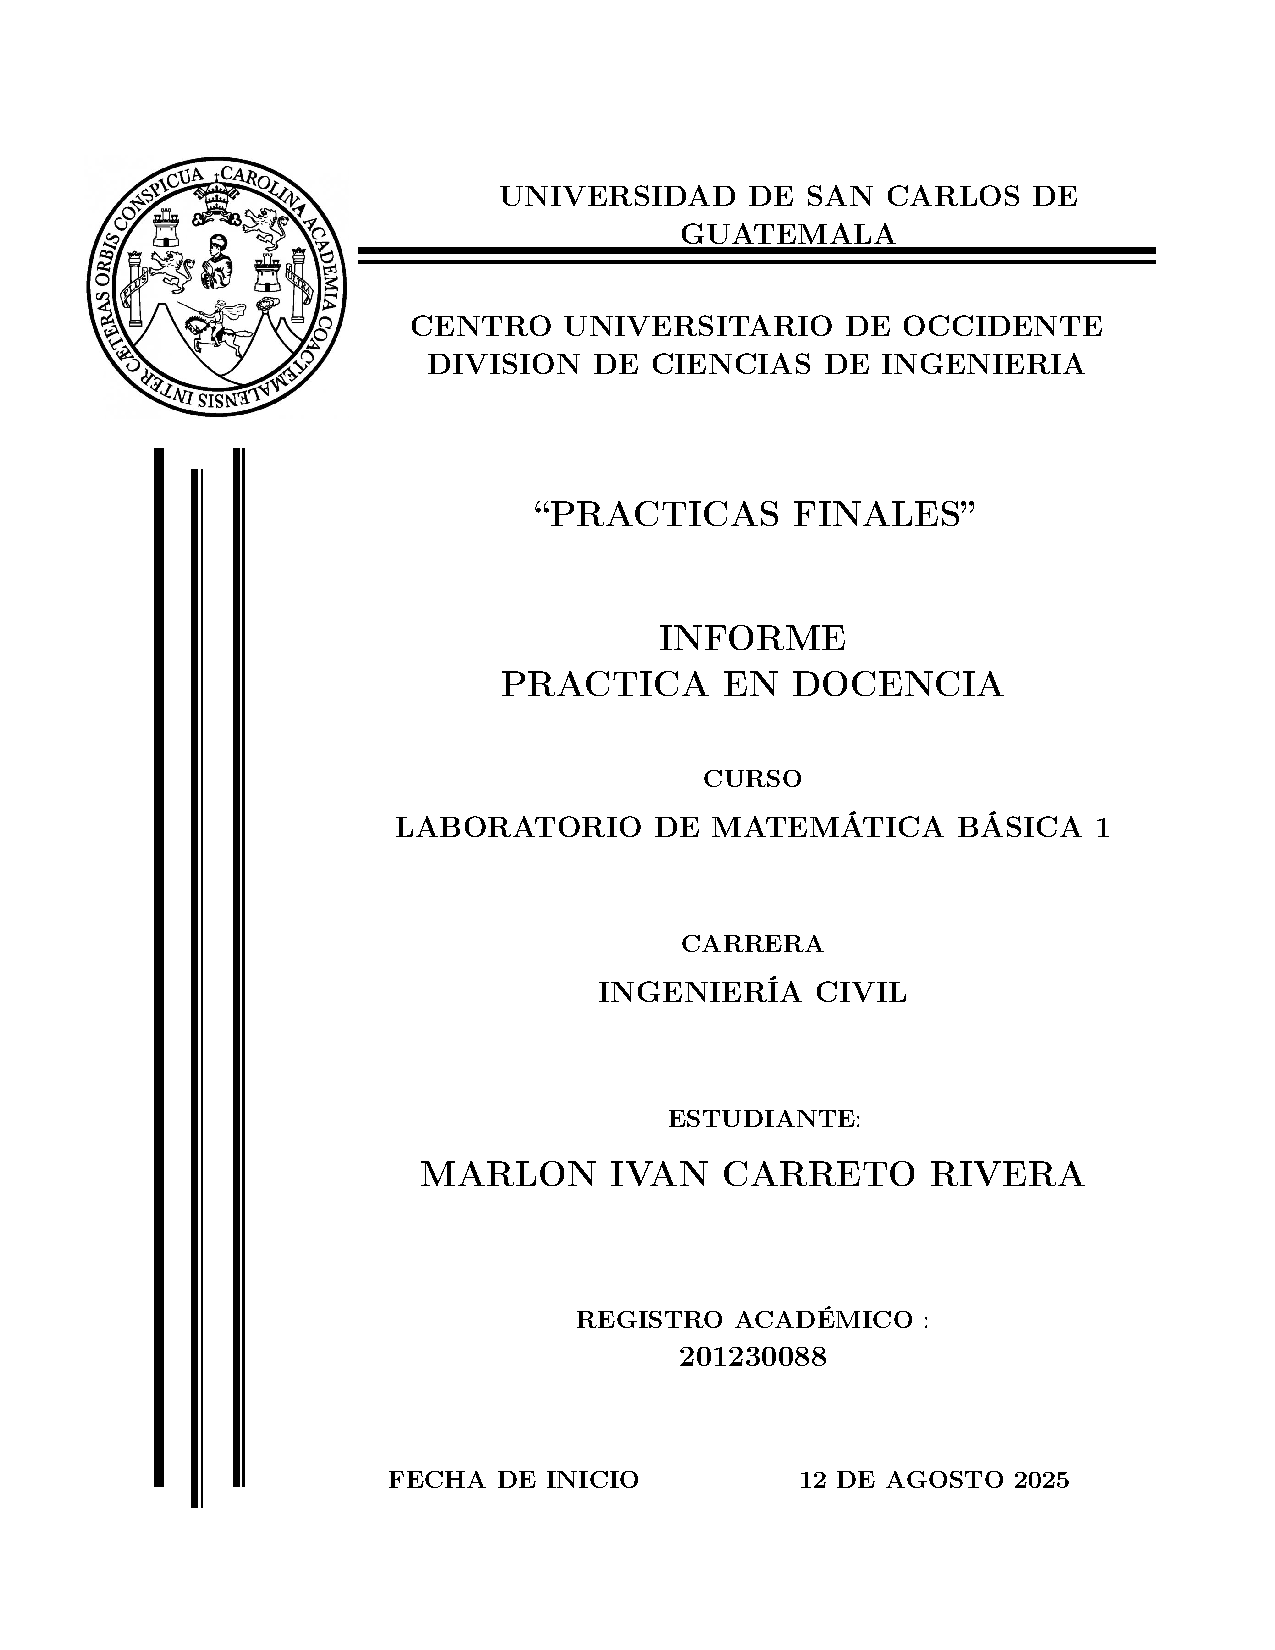
\includepdf{portadaU2D/caratulaUD}
	
	%-------------HOJA ADJUNTA------------
	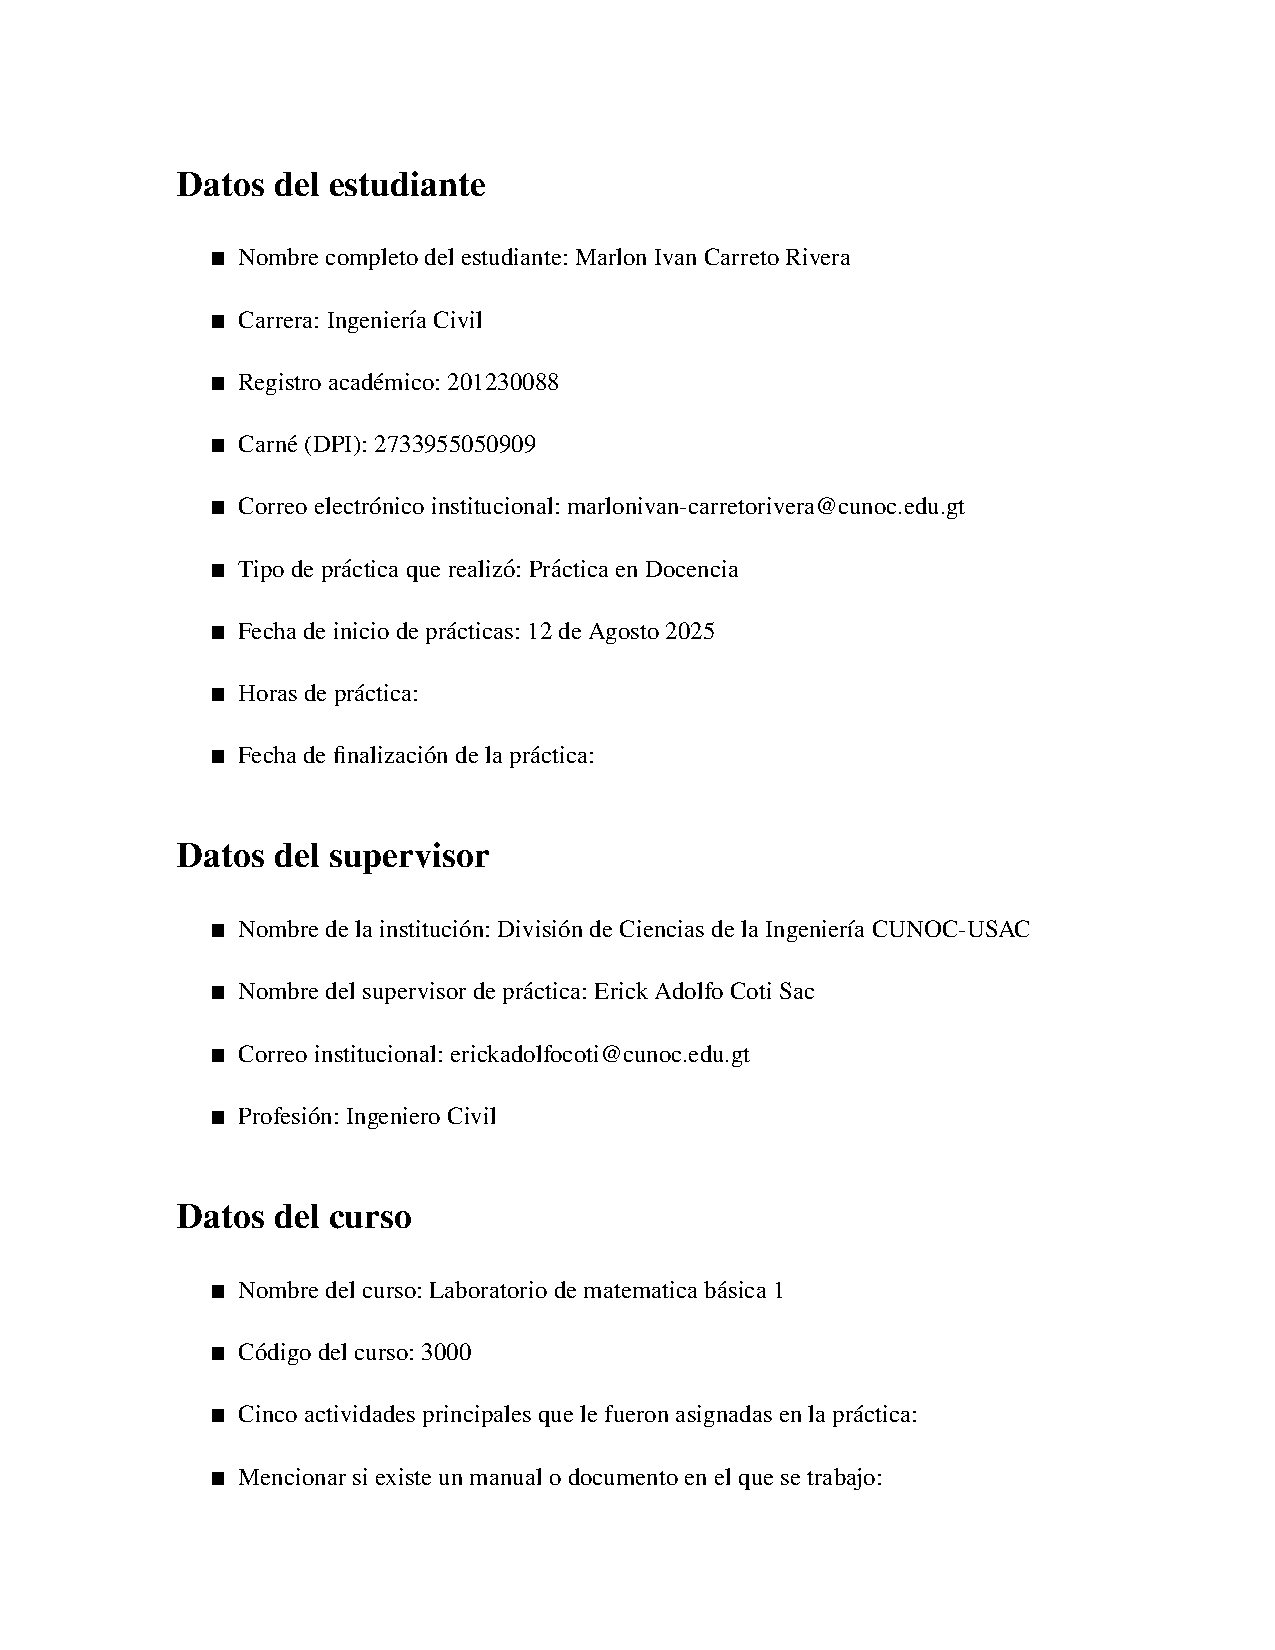
\includepdf[
	pages=-,
	pagecommand={\thispagestyle{empty}}
	]{hojaD/hojaadjuntaD}
	
	

	 
	%------------OFICIO FIRMADO---------
	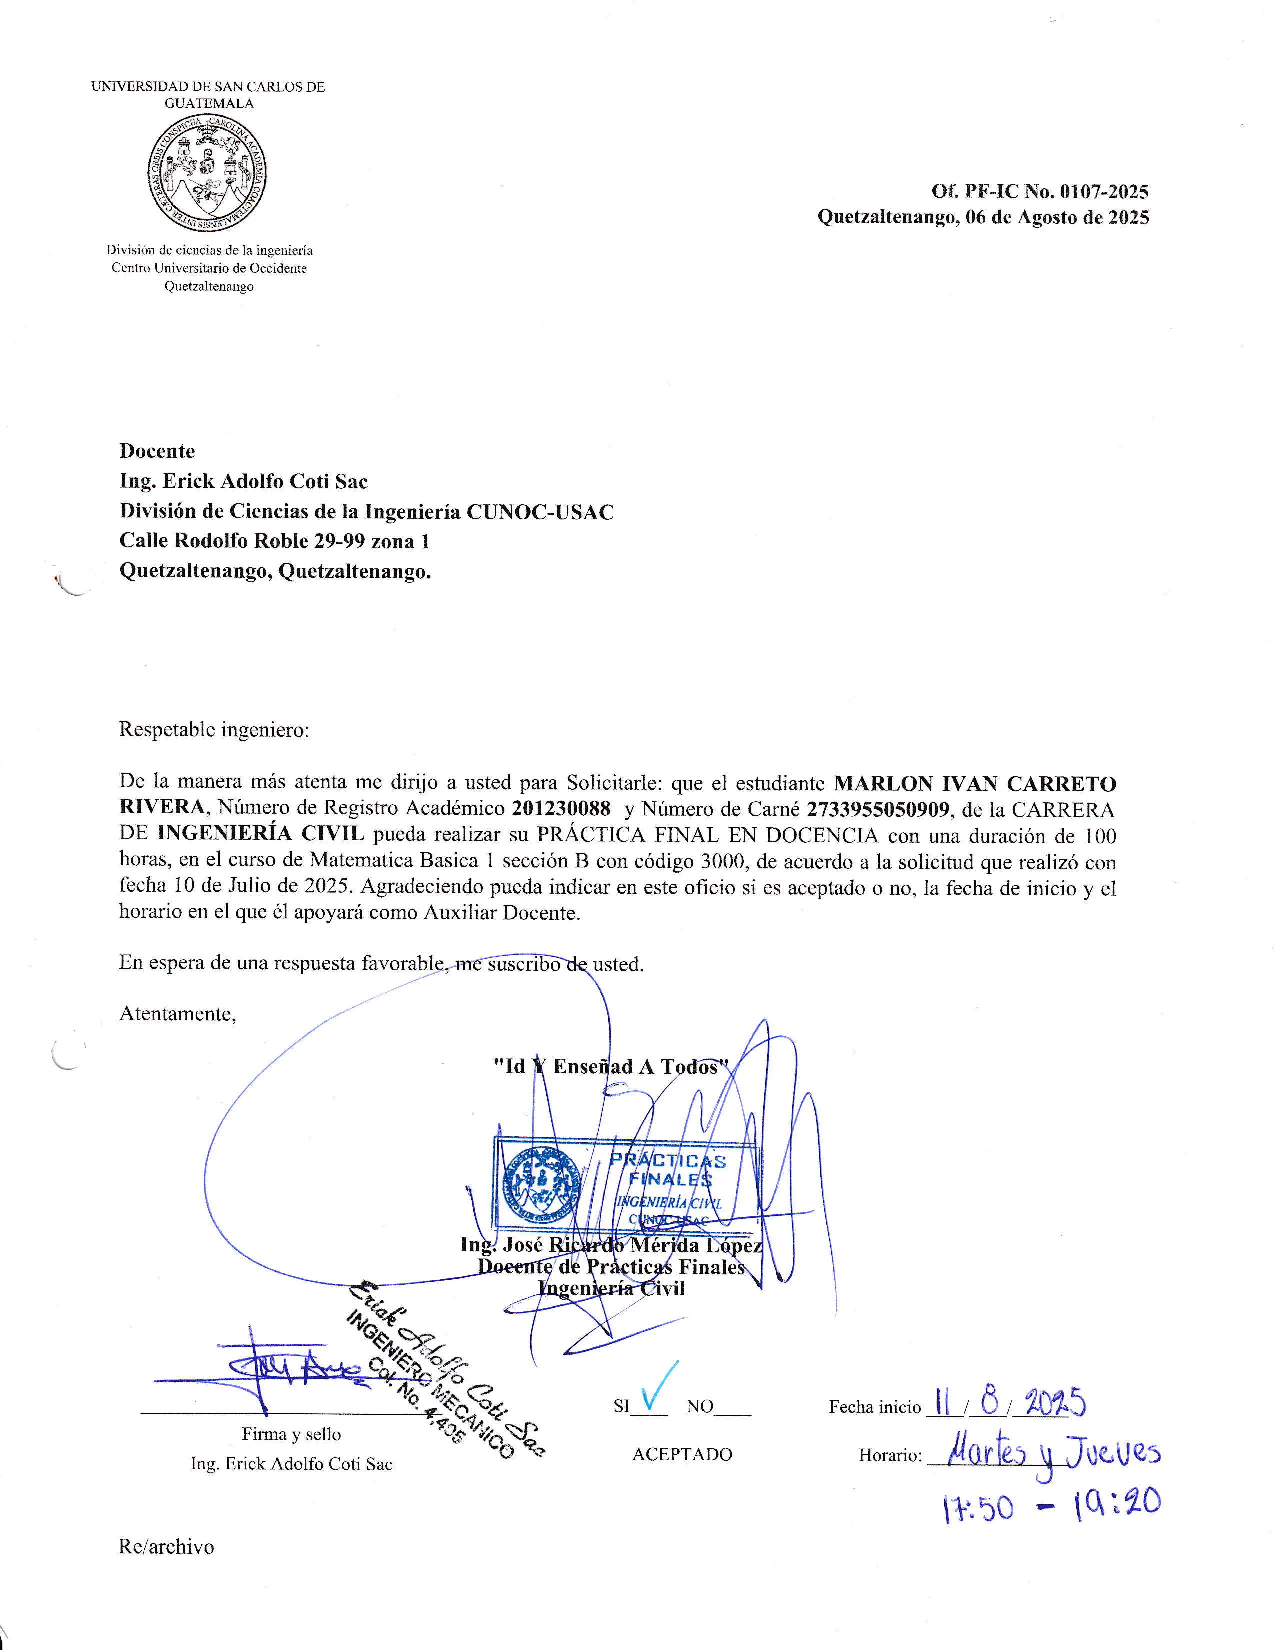
\includepdf{scanerD/oficiofirmadoD}
	
	
	
	%%-------------FINIQUITO-------------
		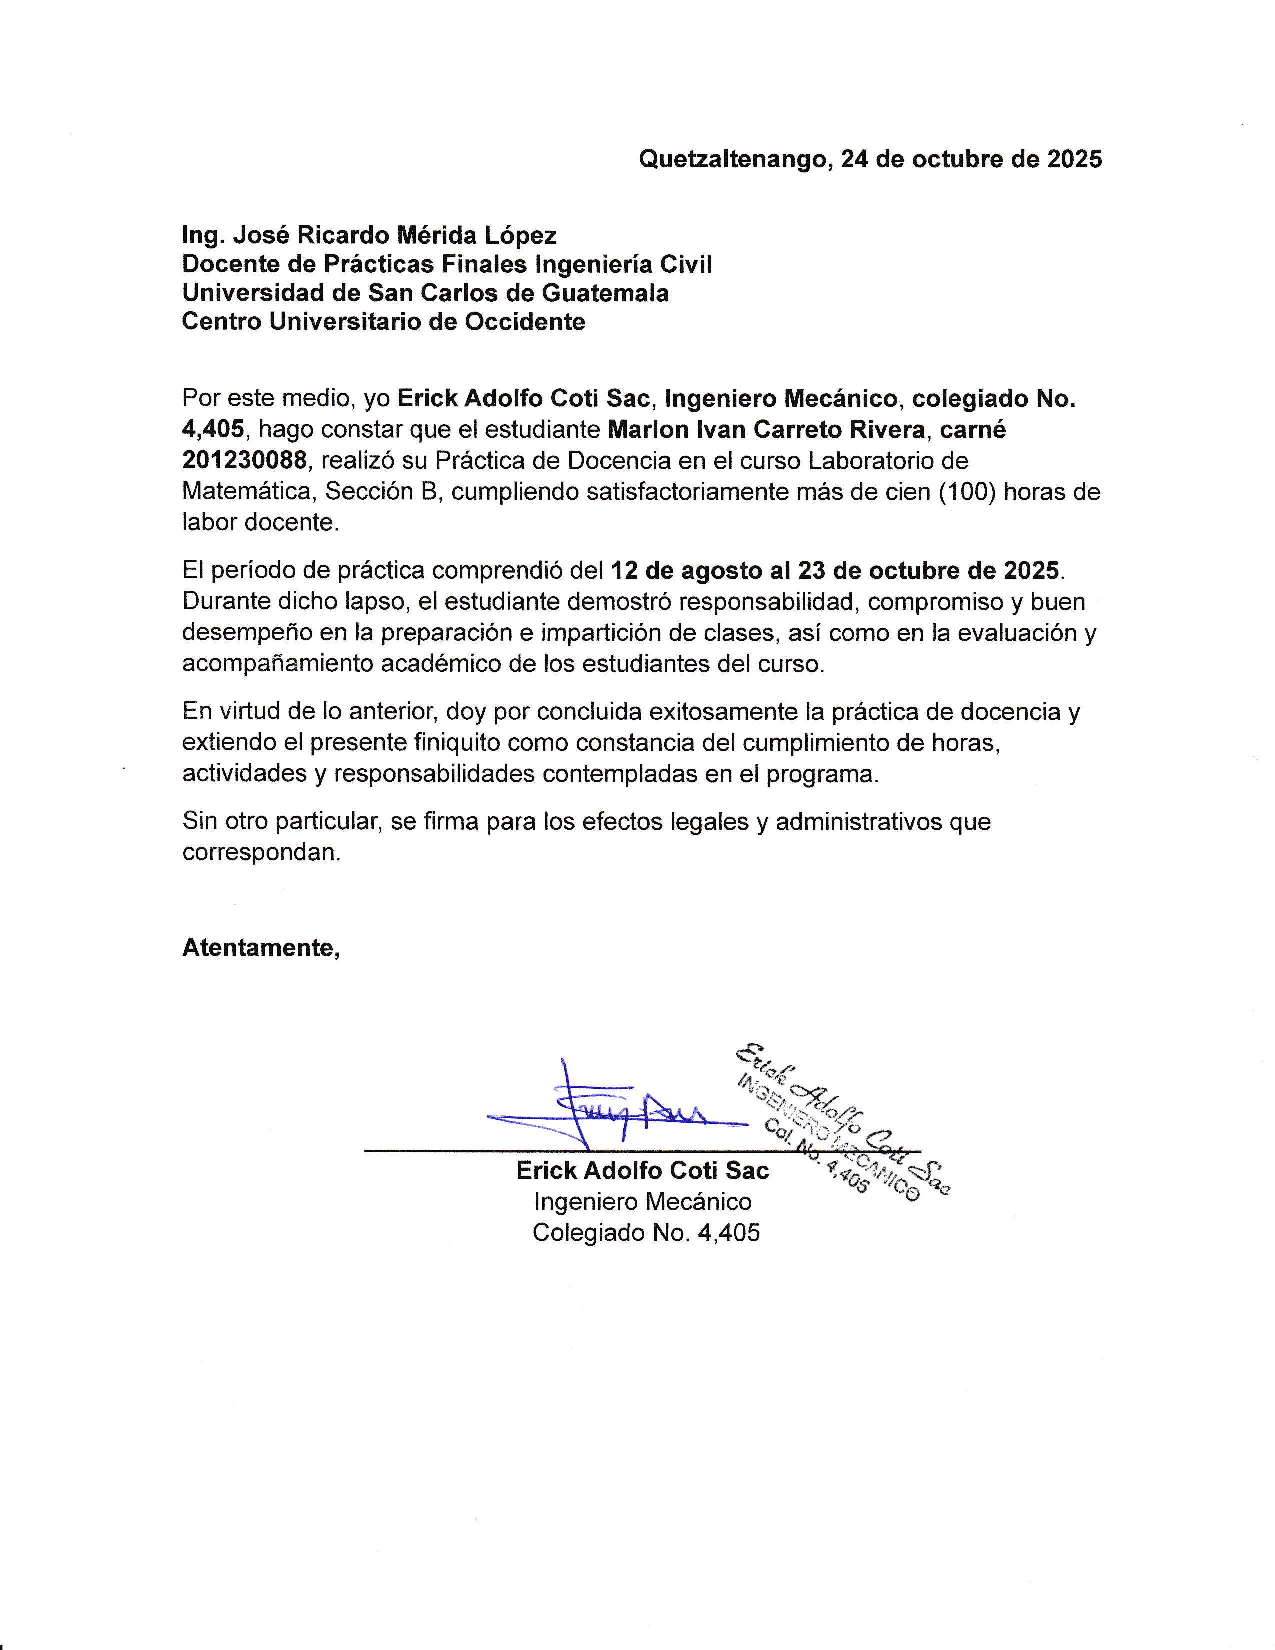
\includepdf{scanerD/finiquitodocencia}
	
	%%-------------BITACORA ESCANEADA----
	
		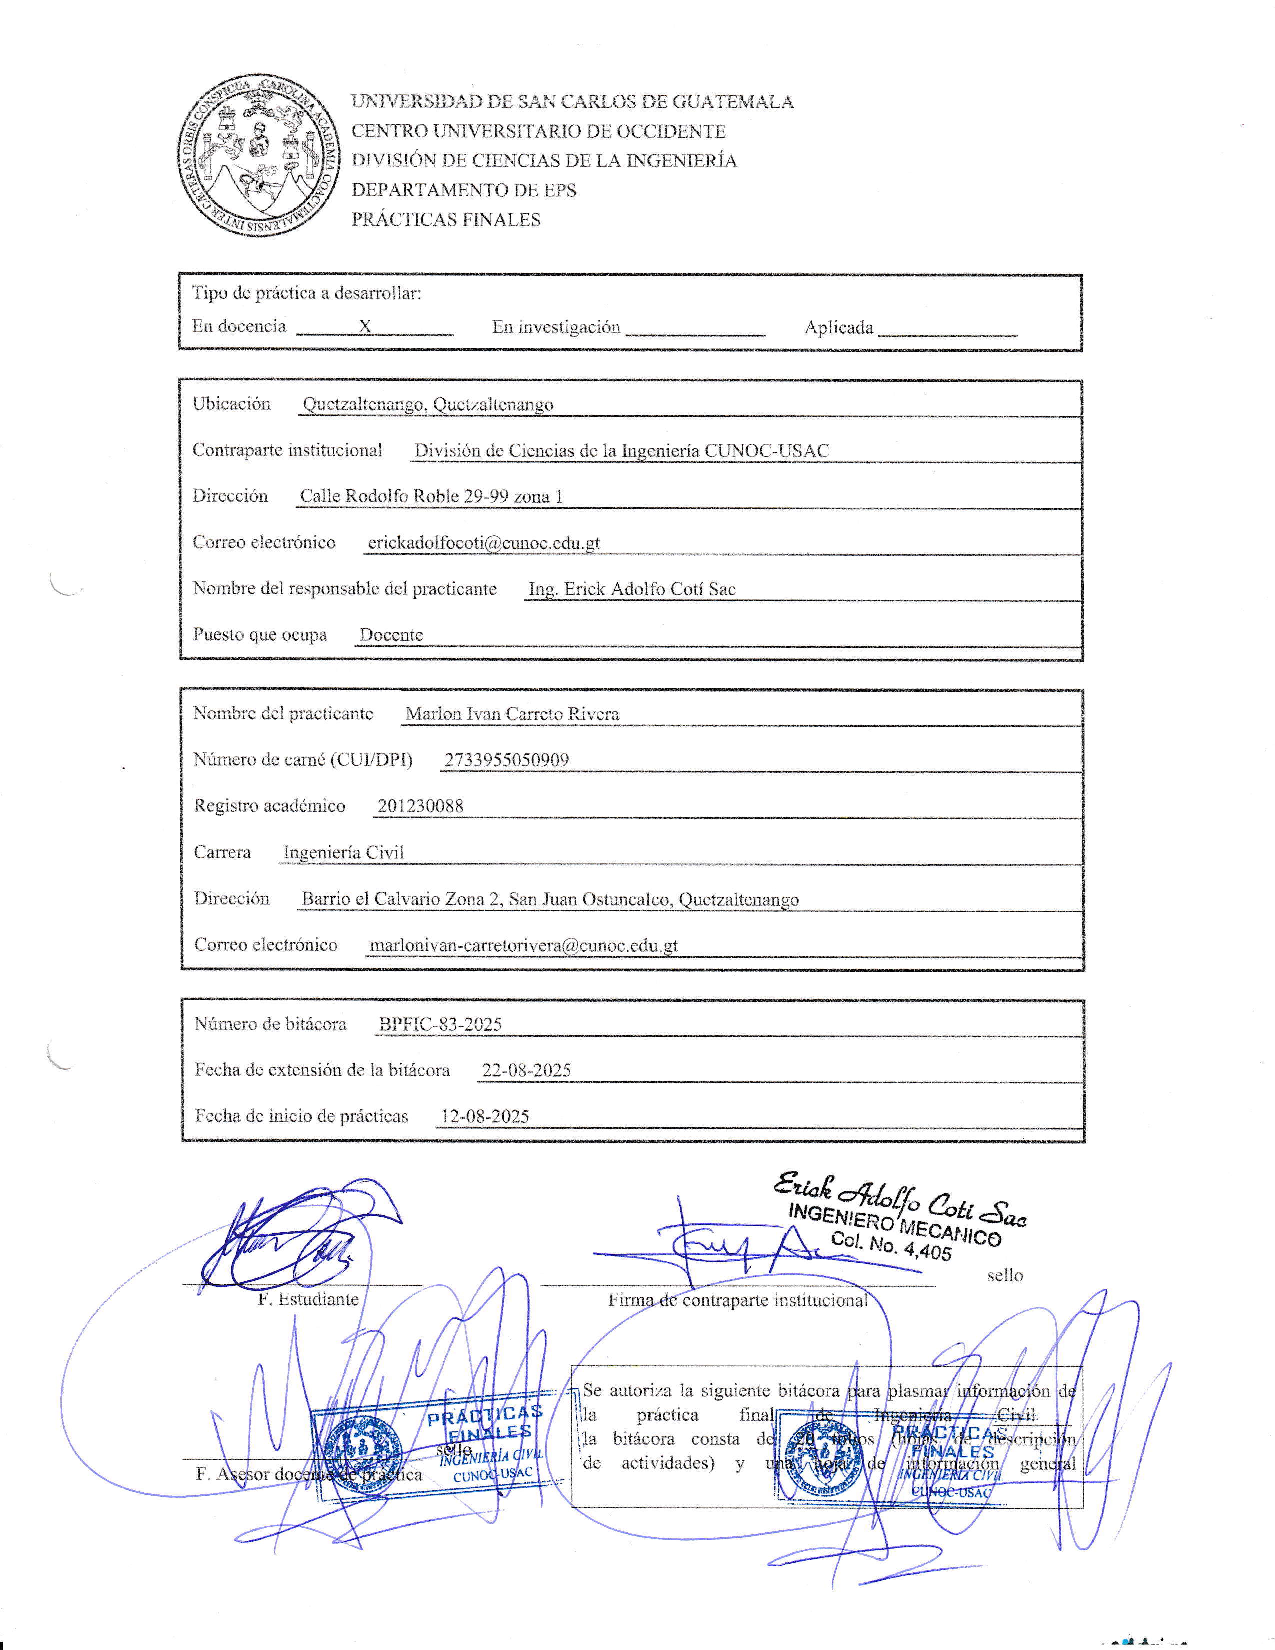
\includepdf[
	pages=-,
	pagecommand={\thispagestyle{empty}}
	]{bitacoradocencia/bitacoradocencia}
	
	%-------------CUERPO DEL INFORME NORMAL
	
	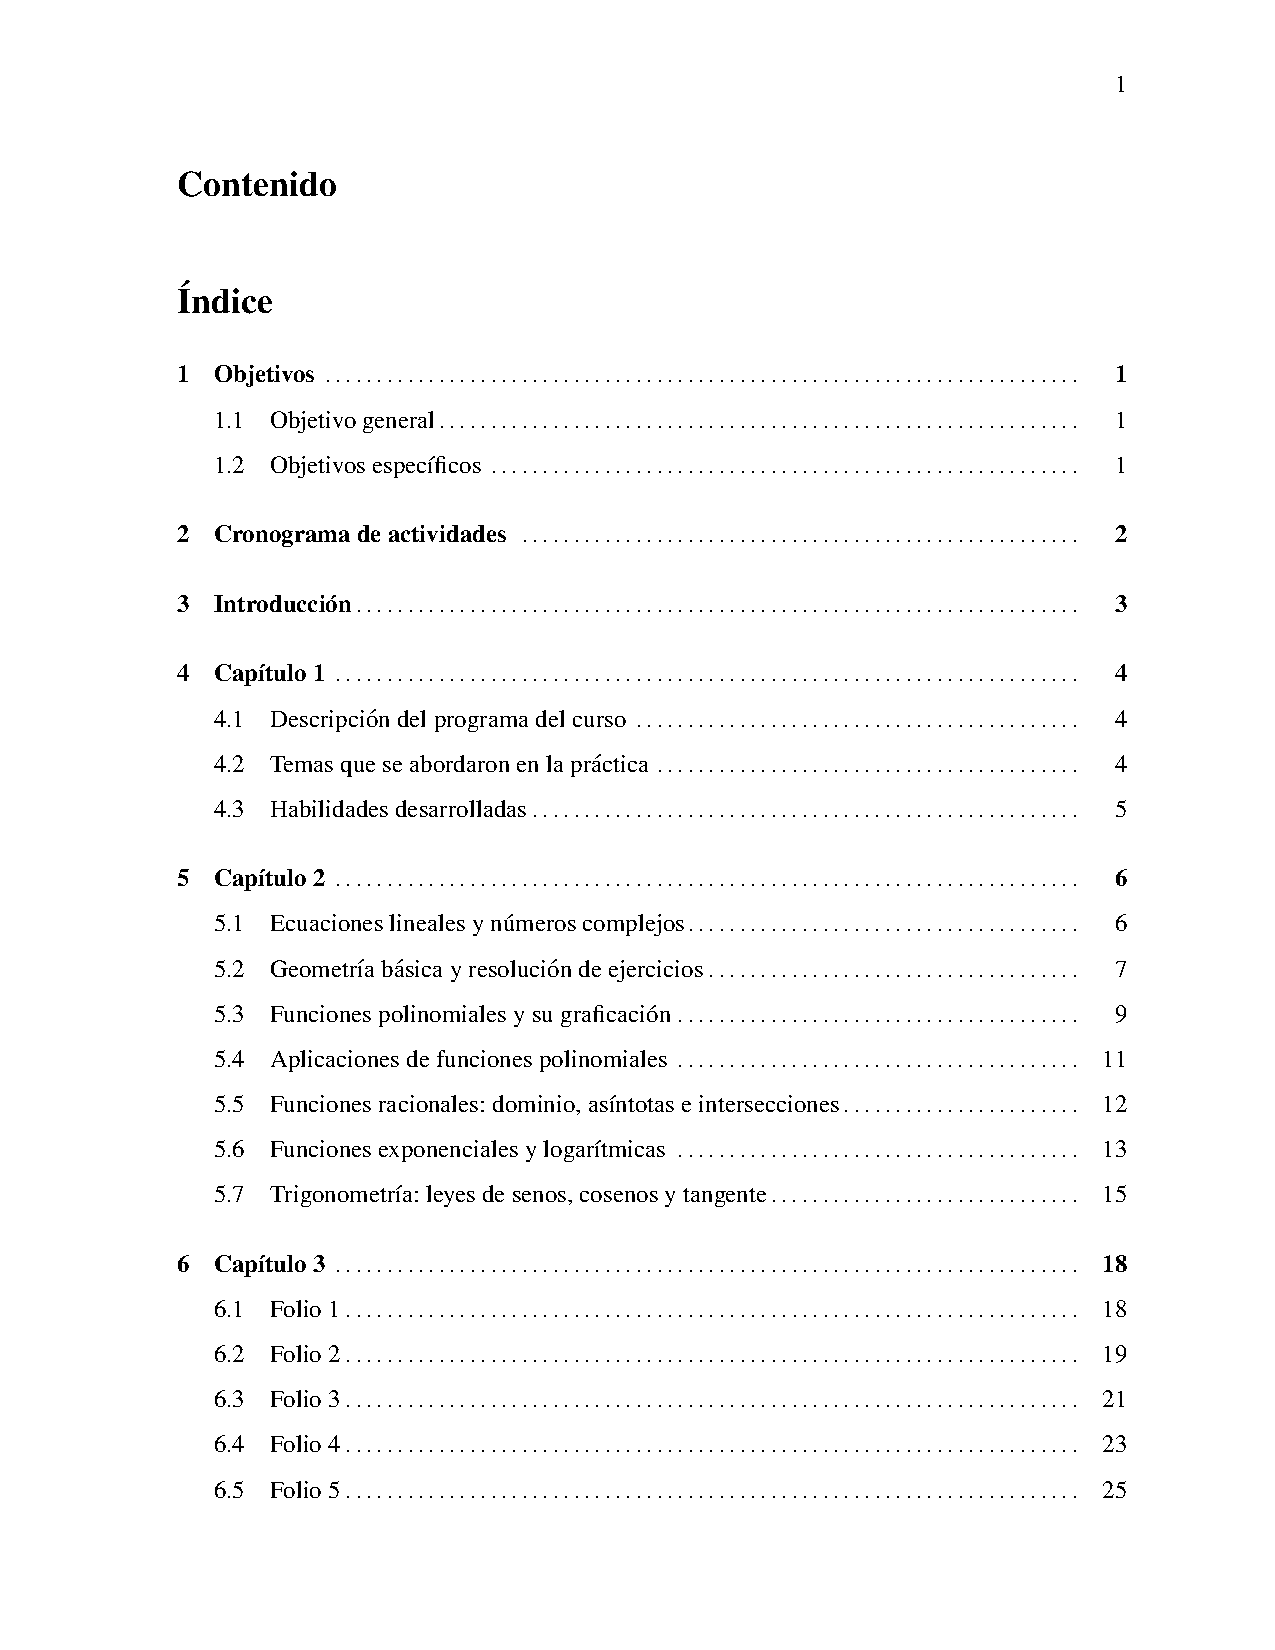
\includepdf[
	pages=-,
	pagecommand={\thispagestyle{empty}}
	]{cuerpoinformeD/cuerpoinformeD}
	


	
		
	
\end{document}